% Provenance (never printed): see sources/outline_sources.md (Year 1: internal
% structure of the Earth from seismology; reference model; density, gravity and
% pressure inside the Earth; mantle mineralogy; lithosphere and asthenosphere).
% Curves from figdata/bachelor-1/prem_profiles.py (shared dataset data:prem) and
% figdata/bachelor-1/refraction.py (generic two-layer crust); exercise and problem
% values in the Book 3 scratch calculator calc/ch09.py.
\chapter{الأرض ذات الطبقات}\label{ch:b1:layered-earth}

في 8 أكتوبر 1909 هزّ زلزال وادي كوبا، جنوب شرقي زغرب.
% ledger: skoko:mohorovicic
جمع أندريا موهوروفيتشيتش، الذي كان يدير المرصد هناك، تسجيلات الزلازل المسجّلة عبر أوروبا، ولاحظ أمرًا غريبًا: حتى مسافة بضع مئات الكيلومترات من المركز السطحي تصل الهزّة الأولى بطريقة، وأبعد من ذلك تحلّ محلّها وصلة أولى من نوع آخر، كأن جزءًا من الطاقة وجد طريقًا أسرع في العمق. وفسّر ذلك بسطح فاصل على عمق نحو خمسين كيلومترًا، تسير الموجات تحته أسرع: قاعدة \omterm{def:b1:layered-earth:layers}{القشرة}. وقد حوّل قرن من هذه التسجيلات، بالملايين، ذلك الحدّ الأول إلى نموذج مرجعي للأرض كلها، طبقةً طبقة، بسرعاتها وكثافتها وجاذبيتها وضغطها حتى المركز. يبيّن هذا الفصل كيف يُعثَر على سطح فاصل من أزمنة السير، وماذا يقول النموذج المرجعي، وكيف يُرسم منحنى الكثافة من السرعات الزلزالية وحدها ويُتحقَّق منه بكتلة الأرض وعزم قصورها الذاتي، وأيّ \omterm{def:b1:rock-forming-minerals:mineral}{المعادن} تكوّن \omterm{def:b1:layered-earth:layers}{الوشاح} عند كل عمق، وممّ يتكوّن اللب، وأين تنتهي \omterm{def:b1:layered-earth:layers}{القشرة} الصلبة الخارجية للكوكب.

\begin{recall}
موجة P موجة ضغط، وموجة S موجة قص؛ فموجات S لا تعبر السوائل، وتعطي منطقتا الظل لموجتي P وS في اللب نصف قطر \omterm{def:b1:layered-earth:layers}{اللب الخارجي} السائل (الكتاب 2، الصف 11). وتنكسر الموجات عند سطح فاصل وفق قانون سنل، $\sin i_1/v_1 = \sin i_2/v_2$ (الفيزياء). وفي مائع ساكن يزداد الضغط مع العمق وفق $\mathrm dP = \rho g\,\mathrm dz$ (من كتاب الفيزياء للسنة الأولى). وقد عُرّفت \omterm{def:b1:layered-earth:layers}{القشرة} \omterm{def:b1:layered-earth:layers}{والوشاح} واللب في الكتاب 1 (الصف 6).
\end{recall}

\section{الموجات الزلزالية في أرض متعددة الطبقات}

تتوقف سرعات الموجات الزلزالية على معاملات مرونة الصخر وعلى كثافته. وتشتقّها كتب الفيزياء من معادلات المرونة للأوساط المتصلة؛ وهنا تُؤخذ معلومةً.

\begin{proposition}[السرعات الزلزالية]\label{prop:b1:layered-earth:speeds}
في جسم صلب مرن متماثل الخواص كثافته $\rho$، ومعامل حجمه $K$، ومعامل قصّه $\mu$، تسير موجات P وS بالسرعتين
\[
  v_P = \sqrt{\frac{K + \tfrac43\mu}{\rho}}, \qquad v_S = \sqrt{\frac{\mu}{\rho}}.
\]
وفي السائل $\mu = 0$، أي $v_S = 0$، ولا تنتشر موجة S.
\end{proposition}
\admitted

بما أن $K$ و$\mu$ موجبان، فإن $v_P > v_S$ دائمًا: ففي \omterm{def:b1:layered-earth:layers}{القشرة} \omterm{def:b1:layered-earth:layers}{والوشاح} في PREM تبلغ $v_P$ نحو $1.8$ إلى $1.9$ مرة قدر $v_S$، وتصل موجات P أولًا. وتزداد السرعتان عادةً مع العمق، لأن الضغط يُقسّي الصخر أكثر مما يضغطه، فتنحني الأشعة راجعةً نحو السطح؛ وعند بضعة أعماق تقفزان فجأة.

\begin{definition}[سطح الانفصال الزلزالي، وموهو، وحدّا اللب–الوشاح واللب الداخلي]
\label{def:b1:layered-earth:discontinuity}
\emph{سطح الانفصال الزلزالي}\index{سطح الانفصال الزلزالي} سطح داخل الأرض تتغيّر عنده السرعات الزلزالية أو الكثافة أو كلاهما فجأة، على سمك صغير مقارنةً بطول الموجة الزلزالية. و\emph{انفصال موهوروفيتشيتش}\index{انفصال موهوروفيتشيتش} (أو \emph{موهو}\index{موهو}) هو قاعدة \omterm{def:b1:layered-earth:layers}{القشرة}، حيث تقفز $v_P$ إلى نحو \qty{8}{km.s^{-1}}. و\emph{حدّ اللب–الوشاح}\index{حدّ اللب–الوشاح} هو السطح بين \omterm{def:b1:layered-earth:layers}{الوشاح} الصلب السيليكاتي \omterm{def:b1:layered-earth:layers}{واللب الخارجي} السائل؛ و\emph{حدّ اللب الداخلي}\index{حدّ اللب الداخلي} هو السطح بين \omterm{def:b1:layered-earth:layers}{اللب الخارجي} السائل \omterm{def:b1:layered-earth:layers}{واللب الداخلي} الصلب.
\end{definition}

\subsection{الانكسار عند حدّ طبقة}

لنأخذ طبقة سمكها $h$ وسرعتها $v_1$، هي \omterm{def:b1:layered-earth:layers}{القشرة}، فوق نصف فضاء سرعته $v_2 > v_1$، هو \omterm{def:b1:layered-earth:layers}{الوشاح}، ومصدرًا على السطح. تصل ثلاث موجات إلى مستقبِل على المسافة $x$. تسير الموجة المباشرة في الطبقة بالسرعة $v_1$. وترتدّ الموجة المنعكسة عن السطح الفاصل. أما الشعاع الذي يصطدم بالسطح الفاصل عند الزاوية الحرجة $i_c$، حيث $\sin i_c = v_1/v_2$، فينكسر محاذيًا له، ويسير في الوسط الأسرع تحته مباشرةً بالسرعة $v_2$، ويرسل الطاقة صاعدةً إلى الطبقة بالزاوية نفسها $i_c$ على امتداد طريقه كله.

\begin{definition}[موجة الرأس، ومسافة التقاطع]\label{def:b1:layered-earth:head-wave}
\emph{موجة الرأس}\index{موجة الرأس} هي الموجة التي تسير محاذية لسطح فاصل بسرعة الوسط الأسرع تحته، وتخرج منه صاعدةً بالزاوية الحرجة. و\emph{مسافة التقاطع}\index{مسافة التقاطع} هي المسافة من المصدر التي تصل بعدها موجة الرأس قبل الموجة المباشرة.
\end{definition}

\begin{theorem}[أزمنة السير فوق أرض من طبقتين]\label{thm:b1:layered-earth:two-layer}
فوق طبقة سمكها $h$ وسرعتها $v_1$ تستند إلى نصف فضاء سرعته $v_2 > v_1$، يعطي مصدر سطحي ومستقبِل سطحي على المسافة $x$:
\[
  t_{\text{مباشرة}} = \frac{x}{v_1}, \qquad
  t_{\text{الرأس}} = \frac{x}{v_2} + \frac{2h\cos i_c}{v_1}
  \quad (x \ge 2h\tan i_c), \qquad \sin i_c = \frac{v_1}{v_2},
\]
وتصل \omterm{def:b1:layered-earth:head-wave}{موجة الرأس} أولًا بعد \omterm{def:b1:layered-earth:head-wave}{مسافة التقاطع}
\[
  x_c = 2h\sqrt{\frac{v_2 + v_1}{v_2 - v_1}}.
\]
\end{theorem}

\begin{proof}
تنزل \omterm{def:b1:layered-earth:head-wave}{موجة الرأس} عبر الطبقة بالزاوية $i_c$، في مسار طوله $h/\cos i_c$، ثم تسير محاذية للسطح الفاصل على مسافة $x - 2h\tan i_c$، وتصعد على مسار طوله $h/\cos i_c$. وزمن سيرها هو
\[
  t_{\text{الرأس}} = \frac{2h}{v_1\cos i_c} + \frac{x - 2h\tan i_c}{v_2}
  = \frac{x}{v_2} + \frac{2h}{v_1\cos i_c}\Bigl(1 - \frac{v_1\sin i_c}{v_2}\Bigr)
  = \frac{x}{v_2} + \frac{2h}{v_1\cos i_c}\,(1 - \sin^2 i_c),
\]
أي $x/v_2 + 2h\cos i_c/v_1$. والمسار موجود فقط إذا كان المدى الأفقي موجبًا، $x \ge 2h\tan i_c$. ويتساوى الزمنان حين $x(1/v_1 - 1/v_2) = 2h\cos i_c/v_1$؛ ومع $\cos i_c = \sqrt{v_2^2 - v_1^2}/v_2$،
\[
  x\,\frac{v_2 - v_1}{v_1 v_2} = \frac{2h\sqrt{(v_2 - v_1)(v_2 + v_1)}}{v_1 v_2},
\]
وهذا يعطي $x_c$. وبعده يقع خط \omterm{def:b1:layered-earth:head-wave}{موجة الرأس}، ذو الميل الأصغر $1/v_2$، تحت خط الموجة المباشرة.
\end{proof}

على مخطط زمن السير بدلالة المسافة، تكون الموجة المباشرة \omterm{def:b1:layered-earth:head-wave}{وموجة الرأس} خطّين مستقيمين. ميلاهما هما السرعتان مقلوبتين، $1/v_1$ و$1/v_2$؛ ويقطع خط \omterm{def:b1:layered-earth:head-wave}{موجة الرأس}، عند امتداده إلى $x = 0$، محور الزمن عند \emph{زمن القطع} $t_i = 2h\cos i_c/v_1$. أما الموجة المنعكسة، $t = \sqrt{x^2 + 4h^2}/v_1$، فقطع زائد يمسّ خط \omterm{def:b1:layered-earth:head-wave}{موجة الرأس} عند المسافة الحرجة $2h\tan i_c$، حيث تنشأ \omterm{def:b1:layered-earth:head-wave}{موجة الرأس} (\cref{exo:b1:layered-earth:10}).

\begin{omfigure}
\begin{tabular}{@{}c@{}}
\begin{tikzpicture}
\begin{axis}[width=0.86\linewidth, axis equal image, xmin=0, xmax=260, ymin=-62, ymax=8,
  axis x line=top, axis y line=left, axis line style={-}, clip=false,
  ylabel={\foreignlanguage{arabic}{العمق \babelsublr{(km)}}}, ytick={-60,-35,0},
  yticklabels={60,35,0}, tick label style={font=\scriptsize}, label style={font=\small}]
\fill[brown!12] (axis cs:0,0) rectangle (axis cs:260,-35);
\fill[orange!18] (axis cs:0,-35) rectangle (axis cs:260,-62);
\draw[black!60] (axis cs:0,-35) -- (axis cs:260,-35);
\addplot[very thick, blue!70!black] table[x=x, y=z, unbounded coords=jump,
  restrict expr to domain={\coordindex}{0:1}] {figdata/out/bachelor-1-refraction-rays.dat};
\addplot[thick, dashed, green!45!black] table[x=x, y=z, unbounded coords=jump,
  restrict expr to domain={\coordindex}{3:5}] {figdata/out/bachelor-1-refraction-rays.dat};
\addplot[very thick, red!75!black] table[x=x, y=z, unbounded coords=jump,
  restrict expr to domain={\coordindex}{7:10}] {figdata/out/bachelor-1-refraction-rays.dat};
\node[font=\scriptsize, anchor=north west] at (axis cs:2,-36) {الوشاح، $v_2 = \qty{8.0}{km.s^{-1}}$};
\node[font=\scriptsize, anchor=center] at (axis cs:125,-17) {القشرة، $v_1 = \qty{6.0}{km.s^{-1}}$، $h = \qty{35}{km}$};
\node[font=\scriptsize, red!75!black, anchor=north] at (axis cs:150,-36) {موجة الرأس على طول موهو};
\node[font=\scriptsize, green!45!black, anchor=south] at (axis cs:40,-20) {منعكسة};
\node[font=\scriptsize, blue!70!black, anchor=north] at (axis cs:125,-1) {مباشرة};
\fill (axis cs:0,0) circle (2pt);
\end{axis}
\end{tikzpicture}\\[2pt]
{\small (أ) مسارات الأشعة (المسافة بالكيلومتر)}\\[6pt]
\begin{tikzpicture}
\begin{axis}[omrecord, width=0.86\linewidth, height=6.0cm, xmin=0, xmax=400, ymin=0, ymax=70,
  xlabel={\foreignlanguage{arabic}{المسافة $x$ \babelsublr{(km)}}}, ylabel={\foreignlanguage{arabic}{زمن السير $t$ \babelsublr{(s)}}}, tick label style={font=\scriptsize},
  label style={font=\small}, clip=false,
  legend style={font=\scriptsize, at={(0.03,0.97)}, anchor=north west, draw=none, fill=white, fill opacity=0.85}]
\addplot[very thick, blue!70!black] table[x=x, y=t_direct] {figdata/out/bachelor-1-refraction-times.dat};
\addlegendentry{مباشرة، ميل $1/v_1$}
\addplot[thick, dashed, green!45!black] table[x=x, y=t_reflected] {figdata/out/bachelor-1-refraction-times.dat};
\addlegendentry{منعكسة}
\addplot[very thick, red!75!black, unbounded coords=jump] table[x=x, y=t_head] {figdata/out/bachelor-1-refraction-times.dat};
\addlegendentry{موجة الرأس، ميل $1/v_2$}
\addplot[thin, dotted, red!75!black, domain=0:79.37] {x/8 + 7.717};
\draw[black!60, densely dashed] (axis cs:185.2,0) -- (axis cs:185.2,30.87);
\node[font=\scriptsize, anchor=north west] at (axis cs:187,8) {$x_c = \qty{185}{km}$};
\node[font=\scriptsize, anchor=east, red!75!black] at (axis cs:-3,7.7) {$t_i$};
\end{axis}
\end{tikzpicture}\\[2pt]
{\small (ب) أزمنة السير}
\end{tabular}
\par\smallskip{\small انكسار عبر \omterm{def:b1:layered-earth:layers}{القشرة} سمكها \qty{35}{km}، بسرعة \qty{6.0}{km.s^{-1}}، فوق \omterm{def:b1:layered-earth:layers}{الوشاح} بسرعة \qty{8.0}{km.s^{-1}} ((أ) بمقياس حقيقي). (أ) تسير الموجة المباشرة على السطح؛ والموجة المنعكسة المرسومة هي التي تصطدم \omterm{def:b1:layered-earth:discontinuity}{بموهو} عند الزاوية الحرجة، \ang{48.6}؛ وتسير \omterm{def:b1:layered-earth:head-wave}{موجة الرأس} على طول \omterm{def:b1:layered-earth:discontinuity}{موهو} وتعود بتلك الزاوية. (ب) أزمنة الوصول: تظهر \omterm{def:b1:layered-earth:head-wave}{موجة الرأس} عند المسافة الحرجة، \qty{79}{km}، مماسّةً للانعكاس، وتسبق الموجة المباشرة عند \omterm{def:b1:layered-earth:head-wave}{مسافة التقاطع}، \qty{185}{km}. والامتداد المنقّط يعطي زمن القطع $t_i = \qty{7.7}{s}$.}
\end{omfigure}

\begin{method}[عمق سطح فاصل من مقطع انكسار]\label{met:b1:layered-earth:moho}
\begin{enumerate}
  \item ارسم أزمنة الوصول الأولى بدلالة المسافة، وركّب خطًا مستقيمًا واحدًا على الوصلات القريبة من المصدر، وآخر على البعيدة.
  \item مقلوبا الميلين يعطيان $v_1$ و$v_2$؛ ثم $\sin i_c = v_1/v_2$.
  \item اقرأ زمن القطع $t_i$ للخط البعيد عند $x = 0$، واحسب $h = t_i v_1/(2\cos i_c)$؛ وتحقّق منه \omterm{def:b1:layered-earth:head-wave}{بمسافة التقاطع}، $h = \tfrac12 x_c\sqrt{(v_2 - v_1)/(v_2 + v_1)}$.
  \item لا يُعثَر على سطح فاصل إلا إذا كان $v_2 > v_1$: فطبقة أبطأ تحت طبقة أسرع لا تعطي موجة رأس، وتبقى مخفية.
\end{enumerate}
\end{method}

كان النوعان الأوليان من وصلات موهوروفيتشيتش هذين الخطين بالضبط: الموجة المباشرة في \omterm{def:b1:layered-earth:layers}{القشرة} قرب المصدر، \omterm{def:b1:layered-earth:head-wave}{وموجة الرأس} على طول أعلى \omterm{def:b1:layered-earth:layers}{الوشاح} أبعد. وقد تأكد ترتيب حجم سمك \omterm{def:b1:layered-earth:layers}{القشرة} في تلك المنطقة الذي قدّره بمقدار \qty{54}{km}، لكن عمق \omterm{def:b1:layered-earth:discontinuity}{موهو} يتفاوت من مكان إلى آخر. فتحت المحيطات لا تتجاوز \omterm{def:b1:layered-earth:layers}{القشرة} نحو \qty{5}{km}؛ وتحت القارات يبلغ متوسطها نحو \qty{30}{km}، وتكون أسمك كثيرًا تحت سلاسل الجبال الكبرى. وقد أخذ PREM، في نموذجه المرجعي، \omterm{def:b1:layered-earth:discontinuity}{موهو} على عمق \qty{11}{km} تحت سطح البحر تحت المحيطات، و\qty{35}{km} تحت القارات.
% ledger: skoko:mohorovicic, usgs:crust-thickness, prem:moho-average

\begin{history}[أندريا موهوروفيتشيتش]
\begin{minipage}[t]{0.76\linewidth}\vspace{0pt}
% ledger: skoko:mohorovicic
أندريا موهوروفيتشيتش (1857–1936) جاء إلى علم الزلازل من علم الأرصاد الجوية: معلّمًا، ثم مديرًا لمرصد زغرب الجوي من 1891 إلى 1921، ونشر آخر دراسة أرصادية له عام 1901. وعلى تسجيلات زلزال وادي كوبا في 8 أكتوبر 1909 وجد زوجين مختلفين من أطوار P وS: قرب المصدر وصلت هزّة أولى من نوع، وأبعد وصلت من نوع آخر، كان قد سار أسرع في العمق. وقراءته لهاتين الوصلتين بوصفهما موجة مباشرة وموجة منكسرة تحت سطح فاصل أعطته السطح الذي يحمل اسمه، وأول قياس لسمك \omterm{def:b1:layered-earth:layers}{القشرة}.
\end{minipage}\hfill
\begin{minipage}[t]{0.2\linewidth}\vspace{0pt}
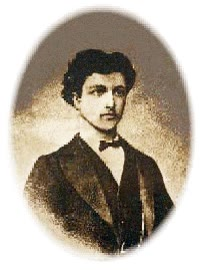
\includegraphics[width=\linewidth]{images/book3/b1-mohorovicic.jpg}

{\scriptsize أندريا موهوروفيتشيتش. ملك عام.}
\end{minipage}
\end{history}

\section{نموذج مرجعي للأرض}

يعطي المنطق نفسه، المطبّق على ملايين أزمنة السير عند كل المسافات وعلى أزمنة الاهتزازات الحرة للأرض (يرنّ الكوكب كله كالجرس بعد زلزال كبير)، السرعات عند كل عمق.

\begin{definition}[نموذج الأرض المرجعي]\label{def:b1:layered-earth:reference-model}
\emph{نموذج الأرض المرجعي}\index{نموذج الأرض المرجعي} أرض متماثلة كرويًا، تُعطى بالسرعات الزلزالية $v_P(r)$ و$v_S(r)$، والكثافة $\rho(r)$، وفي أكمل النماذج التوهين، دوالّ لنصف القطر $r$ وحده؛ وهي تطابق أزمنة السير المرصودة، وأزمنة الاهتزازات الحرة، وكتلة الأرض وعزم قصورها الذاتي. وأكثرها استعمالًا PREM، أي نموذج الأرض المرجعي الأولي (1981).
\end{definition}

صُمّم PREM ليطابق نصف قطر الأرض \qty{6371}{km}، وكتلتها \qty{5.974e24}{kg}، ومعامل عزم القصور الذاتي $0.3308$. وهو يقسّم الكوكب إلى مناطق قليلة تفصل بينها سطوح انفصال، وتُظهر منحنياته (الشكل أدناه) الطبقات الرئيسية في الحال.

\begin{definition}[القشرة، والوشاح، واللب الخارجي، واللب الداخلي]\label{def:b1:layered-earth:layers}
\emph{القشرة}\index{القشرة} هي الطبقة السيليكاتية الخارجية فوق \omterm{def:b1:layered-earth:discontinuity}{موهو}. و\emph{الوشاح}\index{الوشاح} هو الغلاف السيليكاتي الصلب بين \omterm{def:b1:layered-earth:discontinuity}{موهو} \omterm{def:b1:layered-earth:discontinuity}{وحدّ اللب–الوشاح}، على عمق نحو \qty{2891}{km}. و\emph{اللب الخارجي}\index{اللب الخارجي} هو القشرة المعدنية السائلة بين \omterm{def:b1:layered-earth:discontinuity}{حدّ اللب–الوشاح} \omterm{def:b1:layered-earth:discontinuity}{وحدّ اللب الداخلي}، على عمق نحو \qty{5150}{km}. و\emph{اللب الداخلي}\index{اللب الداخلي} هو الكرة المعدنية الصلبة تحته، ونصف قطرها نحو \qty{1220}{km}.
\end{definition}

\begin{omfigure}
\begin{tikzpicture}
\begin{axis}[omrecord, omdepth, width=0.62\linewidth, height=5.4cm, xmin=0, xmax=14, ymin=0, ymax=6371,
  xlabel={\foreignlanguage{arabic}{السرعة \babelsublr{(\unit{km.s^{-1}})} أو الكثافة \babelsublr{(\unit{g.cm^{-3}})}}}, ylabel={\foreignlanguage{arabic}{العمق \babelsublr{(km)}}},
  ytick={0,1000,...,6000}, tick label style={font=\scriptsize}, label style={font=\small},
  clip=false, legend style={font=\scriptsize, at={(0.02,0.80)}, anchor=north west, draw=none, fill=white}]
\addplot[very thick, blue!70!black] table[x=vp, y=depth] {figdata/out/bachelor-1-prem_profiles-profiles.dat};
\addlegendentry{$v_P$}
\addplot[very thick, red!75!black] table[x=vs, y=depth] {figdata/out/bachelor-1-prem_profiles-profiles.dat};
\addlegendentry{$v_S$}
\addplot[very thick, black!70, densely dashed] table[x=rho, y=depth] {figdata/out/bachelor-1-prem_profiles-profiles.dat};
\addlegendentry{$\rho$}
\draw[black!35] (axis cs:0,670) -- (axis cs:14,670) node[right, font=\scriptsize, black] {670 km};
\draw[black!35] (axis cs:0,2891) -- (axis cs:14,2891) node[right, font=\scriptsize, black] {حدّ اللب–الوشاح};
\draw[black!35] (axis cs:0,5149.5) -- (axis cs:14,5149.5) node[right, font=\scriptsize, black] {حدّ اللب الداخلي};
\node[font=\scriptsize, anchor=west] at (axis cs:14,1700) {الوشاح};
\node[font=\scriptsize, anchor=west] at (axis cs:14,4000) {اللب الخارجي (سائل)};
\node[font=\scriptsize, anchor=west] at (axis cs:14,5800) {اللب الداخلي (صلب)};
\end{axis}
\end{tikzpicture}

\par\smallskip{\small PREM: سرعتا موجتي P وS والكثافة بدلالة العمق.
تنعدم سرعة S في \omterm{def:b1:layered-earth:layers}{اللب الخارجي} السائل وتعود صغيرة في
\omterm{def:b1:layered-earth:layers}{اللب الداخلي} الصلب؛ وعند \omterm{def:b1:layered-earth:discontinuity}{حدّ اللب–الوشاح} تكاد الكثافة تتضاعف
بينما تهبط $v_P$ من 13.7 إلى \qty{8.1}{km.s^{-1}}؛ والقفزات قرب
\qty{400}{km} و\qty{670}{km} تحدّ منطقة الانتقال.}
\end{omfigure}

\begin{table}[htbp]
\centering
\footnotesize
\setlength{\tabcolsep}{3pt}
\begin{tabular}{>{\raggedright\arraybackslash}p{0.2\linewidth}rr>{\raggedright\arraybackslash}p{0.47\linewidth}}
\hline
الحدّ في PREM & العمق (km) & نصف القطر (km) & ما الذي يتغيّر \\
\hline
\omterm{def:b1:layered-earth:discontinuity}{موهو} & 24.4 & 6346.6 & \omterm{def:b1:layered-earth:layers}{القشرة} فوقه، والبيريدوتيت تحته؛ $v_P$ من 6.8 إلى 8.1 \\
انفصال عند 220 km & 220 & 6151 & قاعدة المنطقة منخفضة السرعة في PREM \\
انفصال عند 400 km & 400 & 5971 & من \omterm{def:b1:rock-forming-minerals:groups}{الأوليفين} إلى الواداسليت (\qty{410}{km} في معظم الدراسات) \\
انفصال عند 670 km & 670 & 5701 & من الرينغوودايت إلى البريدجمانيت والفيروبيريكلاس (\qty{660}{km} في معظم الدراسات) \\
\omterm{def:b1:layered-earth:discontinuity}{حدّ اللب–الوشاح} & 2891 & 3480 & من السيليكات إلى الحديد السائل؛ $v_S$ من 7.3 إلى 0؛ $\rho$ من 5.57 إلى 9.90 \\
\omterm{def:b1:layered-earth:discontinuity}{حدّ اللب الداخلي} & 5149.5 & 1221.5 & من الحديد السائل إلى الحديد الصلب؛ $v_S$ من 0 إلى 3.5؛ $\rho$ من 12.17 إلى 12.76 \\
\hline
\end{tabular}
\caption{أهم الانفصالات في PREM (السرعات ب\unit{km.s^{-1}}، والكثافات ب\unit{g.cm^{-3}}). يتوسّط PREM \omterm{def:b1:layered-earth:layers}{القشرة} عند \qty{24.4}{km}؛ أما القشور الحقيقية فتتراوح من نحو \qty{5}{km} تحت المحيطات إلى عدة عشرات من الكيلومترات تحت سلاسل الجبال.}
% ledger: usgs:crust-thickness
\label{tab:b1:layered-earth:prem}
\end{table}

حقيقتان في هذه المنحنيات تُلاحظان مباشرة. فانعدام $v_S$ في \omterm{def:b1:layered-earth:layers}{اللب الخارجي} هو ظل موجات S المذكور أعلاه: لا تدخل موجات S اللب إلا بوصفها موجات P، فاللب لا ينقل القصّ، ومن ثم هو سائل. \omterm{def:b1:layered-earth:layers}{واللب الداخلي} ينقل موجات S ببطء: إنه صلب. وجاءت هذه الحقيقة الثانية من وصلات P ضعيفة حيث لا ينبغي أن توجد موجة P.

\begin{history}[إنغه ليمان واللب الداخلي]
% ledger: hjortenberg:lehmann
\begin{minipage}[t]{0.76\linewidth}\vspace{0pt}
إنغه ليمان (1888–1993)، رئيسة قسم علم الزلازل في معهد الجيوديزيا الدنماركي، درست تسجيلات زلزال بولر عام 1929 في نيوزيلندا، فوجدت موجات P تصل داخل منطقة الظل، حيث كان اللب يجب أن يصرفها عنها. وفي بحث عام 1936 بأقصر العناوين، \emph{P$'$}، بيّنت أنها تُفسَّر إذا احتوى اللب على لبّ داخلي أصغر ذي سرعة P أعلى، يعيد جزءًا من الطاقة نحو السطح. ويُعرف الآن أن لبّها الداخلي صلب، وأنه ينمو ببطء مع برودة الأرض. كما اكتشفت الانفصال قرب \qty{220}{km} الذي يحمل اسمها.
\end{minipage}\hfill
\begin{minipage}[t]{0.2\linewidth}\vspace{0pt}
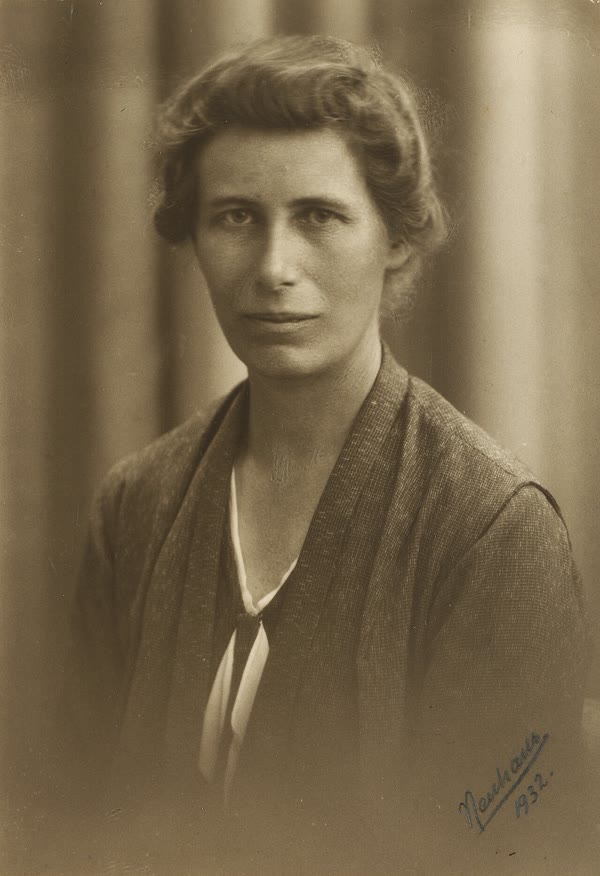
\includegraphics[width=\linewidth]{images/book3/b1-lehmann.jpg}

{\scriptsize إنغه ليمان عام 1932، بتصوير \babelsublr{Even Neuhaus}. ملك عام.}
\end{minipage}
\end{history}

\section{الكثافة والجاذبية والضغط من المعطيات الزلزالية}

تعطي السرعات الزلزالية مزيجين من المعاملات والكثافة، لا الكثافة نفسها. وتأتي علاقة ثالثة من الافتراض بأن الصخر داخل طبقة ذات تركيب متجانس يُضغط ببساطة بوزن الصخر فوقه.

\begin{definition}[المعامل الزلزالي]\label{def:b1:layered-earth:seismic-parameter}
\emph{المعامل الزلزالي}\index{المعامل الزلزالي} عند عمق هو
\[
  \Phi = v_P^2 - \tfrac43 v_S^2 = \frac{K}{\rho},
\]
أي معامل الحجم مقسومًا على الكثافة، محسوبًا من السرعتين الزلزاليتين وحدهما (\cref{prop:b1:layered-earth:speeds}).
\end{definition}

\begin{theorem}[معادلة آدامز–ويليامسون]\label{thm:b1:layered-earth:adams-williamson}
في منطقة ذات تركيب متجانس، في توازن هيدروستاتيكي، تنضغط بطريقة أديباتية، تتغيّر الكثافة مع نصف القطر وفق
\[
  \frac{\mathrm d\rho}{\mathrm dr} = -\frac{\rho(r)\,g(r)}{\Phi(r)},
\]
حيث $g(r)$ هي الجاذبية عند نصف القطر $r$.
\end{theorem}

\begin{proof}
يعطي التوازن الهيدروستاتيكي $\mathrm dP/\mathrm dr = -\rho g$ (التذكير السابق، مع $\mathrm dz = -\mathrm dr$). ويُعرَّف معامل الحجم ب$K = \rho\,\mathrm dP/\mathrm d\rho$ للانضغاط المعني؛ وبالنسبة إلى صخر ذي تركيب ثابت يُضغط دون تبادل حرارة، فإنه معامل الانضغاط الأديباتي الذي تقيسه الموجات الزلزالية، ومن ثم $\mathrm d\rho/\mathrm dP = \rho/K$. وبقاعدة السلسلة،
\[
  \frac{\mathrm d\rho}{\mathrm dr} = \frac{\mathrm d\rho}{\mathrm dP}\,
  \frac{\mathrm dP}{\mathrm dr} = \frac{\rho}{K}\,(-\rho g) = -\frac{\rho g}{K/\rho}
  = -\frac{\rho g}{\Phi}. \qedhere
\]
\end{proof}

تفشل المعادلة عند سطح انفصال، حيث يتغيّر التركيب أو البنية البلورية، وحيثما تنحرف الحرارة عن المنحنى الأديباتي؛ لكنها بين سطوح الانفصال تُفسّر الزيادة المرصودة للكثافة مع العمق تفسيرًا جيدًا جدًا (اللوحة (ج) من الشكل أدناه). وقد بُنيت أولى نماذج الكثافة بالبدء من كثافة أعلى كل منطقة، ثم التكامل نحو الأسفل، وضبط القيم الابتدائية حتى تخرج الكتلة وعزم القصور الذاتي صحيحين. والعددان الكليان هما تكاملان للكثافة.

\begin{proposition}[الكتلة والجاذبية والضغط وعزم القصور الذاتي]
\label{prop:b1:layered-earth:integrals}
لأرض متماثلة كرويًا نصف قطرها $R$ وكثافتها $\rho(r)$، تكون الكتلة داخل نصف القطر $r$، والجاذبية، والضغط، وعزم القصور الذاتي حول محور يمرّ بالمركز،
\[
  m(r) = \int_0^r 4\pi s^2\rho(s)\,\mathrm ds, \quad
  g(r) = \frac{G\,m(r)}{r^2}, \quad
  P(r) = \int_r^R \rho(s)\,g(s)\,\mathrm ds, \quad
  I = \frac{8\pi}{3}\int_0^R \rho(r)\,r^4\,\mathrm dr.
\]
\end{proposition}

\begin{proof}
قشرة رقيقة نصف قطرها $s$ وسمكها $\mathrm ds$ حجمها $4\pi s^2\,\mathrm ds$، ومن ثم التكامل الأول. والجاذبية لجسم متماثل كرويًا خارج نصف قطر هي جاذبية كتلته داخله، مركّزة في المركز، والقشور الواقعة خارج $r$ تجذب بمحصلة صفرية (نظرية القشرة، المقبولة من كتب الفيزياء)؛ ومن ثم $g(r)$. وبتكامل المعادلة الهيدروستاتيكية من السطح، حيث $P = 0$، يُحصل على $P(r)$. أما عزم القصور الذاتي، فإن قشرة كروية رقيقة كتلتها $\mathrm dm$ ونصف قطرها $r$ لها، حول المحاور $x$ و$y$ و$z$، عزومًا مجموعها
$\int (y^2 + z^2) + (z^2 + x^2) + (x^2 + y^2)\,\mathrm dm = 2r^2\,\mathrm dm$؛
وبالتماثل تتساوى الثلاثة، فيكون كل منها $\tfrac23 r^2\,\mathrm dm$. ومع $\mathrm dm = 4\pi r^2\rho\,\mathrm dr$، يعطي جمع القشور $I$.
\end{proof}

لكرة ذات كثافة منتظمة، $I = \tfrac{8\pi}{15}\rho R^5 = 0.4\,MR^2$. ومعامل الأرض $I/MR^2 = 0.3308$ أصغر: فكتلتها متركّزة نحو المركز، وهذه أول حجة على لبّ كثيف. ومحسوبةً من كثافة PREM وحدها، تعطي التكاملات كتلةً قدرها \qty{5.976e24}{kg} (أي أعلى ب\qty{0.06}{\percent} من الكتلة المقيسة \qty{5.972e24}{kg})، ومعاملًا قدره $0.3309$، وضغطًا مركزيًا قدره \qty{364}{GPa}، وهو القيمة المجدولة مع PREM بدقة \qty{0.1}{\percent}.

\begin{omfigure}
\begin{tabular}{@{}c@{\hspace{2mm}}c@{\hspace{2mm}}c@{}}
\begin{tikzpicture}
\begin{axis}[omrecord, omdepth, width=0.35\linewidth, height=7.0cm, xmin=0, xmax=12, ymin=0, ymax=6371,
  xlabel={$g$ (\unit{m.s^{-2}})}, ylabel={\foreignlanguage{arabic}{العمق \babelsublr{(km)}}}, ytick={0,1000,...,6000}, xtick={0,4,8,12},
  tick label style={font=\scriptsize}, label style={font=\small}]
\addplot[very thick, blue!70!black] table[x=g, y=depth] {figdata/out/bachelor-1-prem_profiles-functionals.dat};
\draw[black!35] (axis cs:0,2891) -- (axis cs:12,2891);
\draw[black!35] (axis cs:0,5149.5) -- (axis cs:12,5149.5);
\node[font=\scriptsize, anchor=south west] at (axis cs:0.3,2891) {حدّ اللب–الوشاح};
\node[font=\scriptsize, anchor=south west] at (axis cs:0.3,5149.5) {حدّ اللب الداخلي};
\end{axis}
\end{tikzpicture}
&
\begin{tikzpicture}
\begin{axis}[omrecord, omdepth, width=0.35\linewidth, height=7.0cm, xmin=0, xmax=400, ymin=0, ymax=6371,
  xlabel={$P$ (GPa)}, ytick={0,1000,...,6000}, yticklabels={}, xtick={0,200,400},
  tick label style={font=\scriptsize}, label style={font=\small}]
\addplot[very thick, red!75!black] table[x=P, y=depth] {figdata/out/bachelor-1-prem_profiles-functionals.dat};
\draw[black!35] (axis cs:0,2891) -- (axis cs:400,2891);
\draw[black!35] (axis cs:0,5149.5) -- (axis cs:400,5149.5);
\node[font=\scriptsize, anchor=south west] at (axis cs:150,2891) {\qty{136}{GPa}};
\node[font=\scriptsize, anchor=south east] at (axis cs:290,5149.5) {\qty{329}{GPa}};
\end{axis}
\end{tikzpicture}
&
\begin{tikzpicture}
\begin{axis}[omrecord, omdepth, width=0.35\linewidth, height=7.0cm, xmin=2, xmax=14, ymin=0, ymax=6371,
  xlabel={$\rho$ (\unit{g.cm^{-3}})}, ytick={0,1000,...,6000}, yticklabels={}, xtick={2,6,10,14},
  tick label style={font=\scriptsize}, label style={font=\small},
  legend style={font=\scriptsize, at={(0.97,0.97)}, anchor=north east, draw=none, fill=white}]
\addplot[very thick, black!55] table[x=rho, y=depth] {figdata/out/bachelor-1-prem_profiles-profiles.dat};
\addlegendentry{PREM}
\addplot[only marks, mark=o, mark size=1.4pt, orange!85!black, each nth point=15, unbounded coords=discard]
  table[x=rho_aw, y=depth] {figdata/out/bachelor-1-prem_profiles-adams.dat};
\addlegendentry{آدامز–ويليامسون}
\end{axis}
\end{tikzpicture}
\\[2pt]
{\small (أ) الجاذبية} & {\small (ب) الضغط} & {\small (ج) الانضغاط الذاتي}
\end{tabular}

\par\smallskip{\small داخل الأرض، من PREM. (أ) و(ب) الجاذبية والضغط محسوبان من كثافة PREM ب\cref{prop:b1:layered-earth:integrals}: تبقى الجاذبية قرب \qty{10}{m.s^{-2}} عبر \omterm{def:b1:layered-earth:layers}{الوشاح}، وتبلغ ذروتها \qty{10.7}{m.s^{-2}} عند \omterm{def:b1:layered-earth:discontinuity}{حدّ اللب–الوشاح}، ثم تنعدم في المركز؛ ويبلغ الضغط \qty{136}{GPa} عند \omterm{def:b1:layered-earth:discontinuity}{حدّ اللب–الوشاح}، و\qty{329}{GPa} عند \omterm{def:b1:layered-earth:discontinuity}{حدّ اللب الداخلي}، و\qty{364}{GPa} في المركز. (ج) معادلة آدامز–ويليامسون، المكاملة نحو الأسفل من كثافة PREM عند \qty{771}{km} وعند أعلى \omterm{def:b1:layered-earth:layers}{اللب الخارجي} بسرعات PREM وجاذبيته (الدوائر)، تتبع PREM بدقة \qty{0.2}{\percent}: فهنا تكون الزيادة في الكثافة انضغاطًا لمادة متجانسة؛ أما القفزات فلا.}
\end{omfigure}

وتزداد الجاذبية في النزول عبر \omterm{def:b1:layered-earth:layers}{الوشاح} نتيجةً مباشرةً للّبّ الكثيف: فالكتلة الباقية داخل نصف القطر تتناقص أبطأ من $r^2$. وعبر \omterm{def:b1:layered-earth:layers}{الوشاح} تكاد $g$ لا تتغيّر، ويزداد الضغط تقريبًا خطيًا مع العمق، بنحو \qty{4.7}{GPa} لكل مئة كيلومتر.


\section{الوشاح: صخر واحد وتجمّعات معدنية عدة}

\omterm{def:b1:layered-earth:layers}{الوشاح} العلوي بيريدوتيت، يُعرف من الكتل التي تحملها البراكين إلى السطح ومن شرائح \omterm{def:b1:layered-earth:layers}{الوشاح} المدفوعة فوق القارات: نحو النصف إلى ثلاثة أخماس \omterm{def:b1:rock-forming-minerals:groups}{أوليفين} بالحجم (\qtyrange{49}{62}{\percent} في التراكيب المقترحة)، والباقي بيروكسينات \omterm{def:b1:rock-forming-minerals:mineral}{ومعدن} غني بالألومنيوم (\omterm{def:b1:rock-forming-minerals:groups}{البلاجيوكلاز}، أو السبينل، أو \omterm{def:b1:rock-forming-minerals:groups}{الجارنيت}، حسب العمق). والضغط المتزايد مع العمق لا يغيّر هذا التركيب، لكنه يُجبر ذراته على تراصّ أكثف: فتظهر المتعددات الأشكال (\cref{ch:b1:rock-forming-minerals}) واحدةً بعد الأخرى.

\begin{definition}[منطقة الانتقال في الوشاح]\label{def:b1:layered-earth:transition-zone}
\emph{منطقة الانتقال في الوشاح}\index{منطقة الانتقال في الوشاح} هي الجزء من \omterm{def:b1:layered-earth:layers}{الوشاح} بين سطحي الانفصال الزلزاليين قرب \qty{410}{km} و\qty{660}{km} من العمق، حيث يُستبدل \omterm{def:b1:rock-forming-minerals:groups}{الأوليفين} في \omterm{def:b1:layered-earth:layers}{الوشاح} العلوي بمتعدّداته الأشكال الأكثف: الواداسليت، ثم الرينغوودايت. فوقها \omterm{def:b1:layered-earth:layers}{الوشاح} العلوي؛ وتحتها \omterm{def:b1:layered-earth:layers}{الوشاح} السفلي، حتى \omterm{def:b1:layered-earth:discontinuity}{حدّ اللب–الوشاح}.
\end{definition}

عند نحو \qty{410}{km} (\qty{14}{GPa}) يتحوّل \omterm{def:b1:rock-forming-minerals:groups}{الأوليفين} \ce{(Mg,Fe)2SiO4} إلى الواداسليت، ذي الصيغة نفسها؛ وقرب \qty{520}{km} (\qty{17.5}{GPa}) يتحوّل الواداسليت إلى الرينغوودايت؛ وتذوب البيروكسينات في \omterm{def:b1:rock-forming-minerals:groups}{جارنيت} غني بالسيليكون، هو المايجوريت، حتى يحوي \omterm{def:b1:rock-forming-minerals:groups}{الجارنيت} عند منتصف منطقة الانتقال كلها، فتكون المنطقة أكثر قليلًا من نصفها متعددات أشكال \omterm{def:b1:rock-forming-minerals:groups}{الأوليفين} والباقي \omterm{def:b1:rock-forming-minerals:groups}{جارنيت}. وعند نحو \qty{660}{km}، عند ضغط قرب \qty{24}{GPa}، ينقسم الرينغوودايت إلى
معدنين، يُكتبان للطرف الطرفي المغنيسيومي:
\[
  \ce{Mg2SiO4 -> MgSiO3 + MgO}:
\]
البريدجمانيت، \ce{(Mg,Fe)SiO3} ذو بنية البيروفسكيت، والفيروبيريكلاس، \ce{(Mg,Fe)O}. ويكون \omterm{def:b1:layered-earth:layers}{الوشاح} السفلي، بالتركيب نفسه \omterm{def:b1:layered-earth:layers}{للوشاح} العلوي، نحو \qty{75}{\percent} بريدجمانيت، و\qty{17}{\percent} فيروبيريكلاس، و\qty{8}{\percent} من بيروفسكيت سيليكات الكالسيوم بالحجم، ويطابق كثافات النموذج المرجعي وسرعاته. ولذلك فالبريدجمانيت هو \omterm{def:b1:rock-forming-minerals:mineral}{المعدن} الأوفر في الأرض؛ ولم يُسمَّ إلا عام 2014، بعد أن وُصفت حبيبات طبيعية في نيزك تعرّض لصدمة شديدة.
% ledger: frost:mantle-transitions, sun:lower-mantle, tschauner:bridgmanite
كل تحوّل ينتج \omterm{def:b1:rock-forming-minerals:mineral}{معادن} أكثف، فيرفع الكثافة والسرعات الزلزالية: والتحوّلات هي سطوح الانفصال في المنحنيات (الشكل أدناه). وأعماقها ليست ثابتة. فالتحوّل الطوري يحدث عند ضغط يتوقف على الحرارة، وميل هذا التوقف (ميل كلابيرون، الذي يُعالَج في المجلد الجامعي التالي) يرفع انفصال \qty{410}{km} ويخفض انفصال \qty{660}{km} في الصخر البارد لصفيحة غائصة. ورسم طبوغرافيا سطوح الانفصال طريقة لتعيين المناطق الباردة والحارة في \omterm{def:b1:layered-earth:layers}{الوشاح}.

\begin{omfigure}
\begin{tikzpicture}[x=0.075mm, y=-0.062mm, font=\scriptsize]
% schematic volume fractions (ledger frost:mantle-transitions, sun:lower-mantle)
\def\W{1000}
% upper mantle 0-410: olivine 60, pyroxenes 30, garnet 10
\fill[green!45!olive!60] (0,0) rectangle (600,410);
\fill[brown!35] (600,0) rectangle (900,410);
\fill[red!35] (900,0) rectangle (1000,410);
% 410-520 wadsleyite 60, garnet 40 ; 520-660 ringwoodite 60, garnet 40
\fill[teal!50] (0,410) rectangle (600,520);
\fill[blue!35] (0,520) rectangle (600,660);
\fill[red!45] (600,410) rectangle (1000,660);
% 660-1000 bridgmanite 75, ferropericlase 17, Ca-perovskite 8
\fill[orange!45] (0,660) rectangle (750,1000);
\fill[gray!40] (750,660) rectangle (920,1000);
\fill[yellow!50] (920,660) rectangle (1000,1000);
\draw (0,0) rectangle (1000,1000);
\foreach \d in {410,520,660} \draw[thick] (0,\d) -- (1000,\d);
\node at (300,205) {الأوليفين};
\node[align=center] at (750,205) {البيروكسينات};
\node[rotate=90] at (950,205) {الجارنيت};
\node at (300,465) {الواداسليت};
\node at (300,590) {الرينغوودايت};
\node[align=center] at (800,590) {الجارنيت};
\node at (375,830) {البريدجمانيت};
\node[rotate=90, align=center] at (835,830) {الفيروبيريكلاس};
\node[rotate=90] at (960,830) {بيروفسكيت الكالسيوم};
\foreach \d in {0,200,410,520,660,800,1000} \node[anchor=east] at (-10,\d) {\d};
\node[rotate=90, anchor=south] at (-160,500) {العمق (km)};
\foreach \p in {0,25,50,75,100} \node[anchor=north] at (\p*10,1010) {\p};
\node[anchor=north] at (500,1080) {النسبة الحجمية المئوية};
\node[anchor=west, align=left] at (1030,205) {الوشاح العلوي};
\node[anchor=west, align=left] at (1030,535) {منطقة\\الانتقال};
\node[anchor=west, align=left] at (1030,830) {الوشاح السفلي};
\end{tikzpicture}

\par\smallskip{\small \omterm{def:b1:rock-forming-minerals:mineral}{المعادن} في \omterm{def:b1:layered-earth:layers}{وشاح} بيريدوتيتي بدلالة العمق، كنسب حجمية (تخطيطي: الحدود مرسومة حادّة، والنسب قيم مدوّرة ضمن المجالات المذكورة في النص). التركيب لا يتغيّر؛ أما \omterm{def:b1:rock-forming-minerals:mineral}{المعادن} فتتغيّر، عند نحو 410 و\num{520} و\qty{660}{km}.}
\end{omfigure}

في قاع \omterm{def:b1:layered-earth:layers}{الوشاح} تتميّز الطبقة المسماة D$''$ (دال مزدوجة، اسم حُفظ من نموذج مبكر للأرض) بتدرّج سرعي مختلف عن بقية \omterm{def:b1:layered-earth:layers}{الوشاح} السفلي؛ ويجعلها PREM أدنى \qty{150}{km} من \omterm{def:b1:layered-earth:layers}{الوشاح}. وهي غير متجانسة زلزاليًا: بقع ذات سرعة منخفضة جدًا، وتدرجات حادة، وعاكسات. ويُظن أنها طبقة حدّية بين اللب الساخن \omterm{def:b1:layered-earth:layers}{والوشاح}، وربما مقبرة للصفائح القديمة.
% ledger: prem:dpp

\section{اللب}

اللب معظمه حديد. فكثافته وسرعاته وقدرته على توليد مجال مغناطيسي كلها تشير إلى \omterm{def:b1:rock-forming-minerals:mineral}{معدن}، والحديد هو العنصر الأوفر بفارق كبير بين العناصر الكثيفة بما يكفي التي تُظهرها النيازك والشمس شائعةً. ويرافقه النيكل، الوفير في النيازك الحديدية. لكن اللب ليس حديدًا ونيكلًا نقيين.
\begin{itemize}
  \item اللب أخفّ بنسبة \qtyrange{5}{10}{\percent} من الحديد النقي لو كان عند الضغط والحرارة نفسيهما: فلا بدّ أن يحوي عناصر خفيفة، والمرشحون منها السيليكون والكبريت والكربون والأكسجين والهيدروجين.
  \item تقفز الكثافة بنحو \qty{4.5}{\percent} عند \omterm{def:b1:layered-earth:discontinuity}{حدّ اللب الداخلي}، وهي قفزة أكبر من أن تنجم عن تجمّد \omterm{def:b1:rock-forming-minerals:mineral}{المعدن} نفسه: \omterm{def:b1:layered-earth:layers}{فاللب الداخلي} يحوي عناصر خفيفة هو الآخر، لكن أقل، بنسبة بضعة بالمئة مقابل \qtyrange{5}{10}{\percent} في السائل.
\end{itemize}
% ledger: badro:core
للفرق نتيجة. فمع برودة الأرض — يبرد وشاحها بنحو \qty{100}{\degreeCelsius} كل مليار سنة حاليًا — يتجمّد سائل اللب على \omterm{def:b1:layered-earth:layers}{اللب الداخلي}، فينمو، ويُبقي التجمّد معظم العناصر الخفيفة في السائل.
% ledger: bellini:cooling
ويصعد السائل الخفيف المنطلق من قاع \omterm{def:b1:layered-earth:layers}{اللب الخارجي}، ويُظنّ أن هذه الطفوية تساعد في تحريك \omterm{def:b1:layered-earth:layers}{اللب الخارجي} وتشغيل الدينامو الذي يولّد المجال المغناطيسي للأرض.

\section{الطبقات الميكانيكية: الغلاف الصخري والغلاف اللدن}

الطبقات أعلاه تُعرَّف بالتركيب والطور: \omterm{def:b1:layered-earth:layers}{فالقشرة} \omterm{def:b1:layered-earth:layers}{والوشاح} صخران مختلفان، \omterm{def:b1:layered-earth:layers}{واللب الخارجي} \omterm{def:b1:layered-earth:layers}{واللب الداخلي} حالتان مختلفتان. أما تكتونية الصفائح فتحتاج تقسيمًا آخر، بحسب المتانة، يقطع التقسيم الأول.

\begin{definition}[الغلاف الصخري، والغلاف اللدن، ومنطقة السرعة المنخفضة]
\label{def:b1:layered-earth:lithosphere}
\emph{الغلاف الصخري}\index{الغلاف الصخري} هو \omterm{def:b1:layered-earth:layers}{القشرة} الصلبة الخارجية للأرض، أي \omterm{def:b1:layered-earth:layers}{القشرة} وأعلى \omterm{def:b1:layered-earth:layers}{الوشاح}، وهو يسلك سلوك طبقة قوية عبر الأزمنة الجيولوجية، وينقسم إلى صفائح. و\emph{الغلاف اللدن}\index{الغلاف اللدن} هو الطبقة الأضعف من \omterm{def:b1:layered-earth:layers}{الوشاح} العلوي تحته، التي تتشوّه بتدفّق بطيء وتتيح للصفائح أن تتحرّك. و\emph{منطقة السرعة المنخفضة}\index{منطقة السرعة المنخفضة} هي نطاق العمق تحت الغلاف الصخري حيث تكون السرعات الزلزالية، وسرعات S خاصةً، أدنى مما فوقه وتحته.
\end{definition}

\omterm{def:b1:layered-earth:lithosphere}{الغلاف الصخري} ليس صخرًا، بل نطاق حرارة: فبيريدوتيت \omterm{def:b1:layered-earth:layers}{الوشاح} قوي حيث يكون باردًا، ويزحف حيث يكون ساخنًا، وقاعدته تقريبًا متساوية الحرارة. وهو رقيق تحت الحيود، حيث يصعد \omterm{def:b1:layered-earth:layers}{الوشاح} الساخن، ويبلغ سمكه نحو \qty{140}{km} تحت أقدم قاع محيطي، و\qtyrange{40}{280}{km} تحت القارات، وأكبرها تحت الكراتونات القديمة؛ ويقع أعلى \omterm{def:b1:layered-earth:lithosphere}{الغلاف اللدن} على نحو \qtyrange{80}{200}{km}. وزلزاليًا يظهر \omterm{def:b1:layered-earth:lithosphere}{الغلاف اللدن} على هيئة \omterm{def:b1:layered-earth:lithosphere}{منطقة السرعة المنخفضة}، قريبًا من شروط انصهاره: ففي PREM تنخفض سرعة S قليلًا من \omterm{def:b1:layered-earth:discontinuity}{موهو} حتى \qty{220}{km}، حيث تقفز ثانيةً. وكيف تتوقف المتانة على الحرارة، ولماذا، موضوع \cref{ch:b1:stress-strain-rheology}.

\begin{inthefield}[محطة زلزالية]
\begin{minipage}[t]{0.55\linewidth}\vspace{0pt}
تأتي أزمنة السير التي تقوم عليها النماذج المرجعية من محطات دائمة. ويقف مقياس الزلازل عريض النطاق، الذي يسجّل حركات الأرض من أجزاء من مئة من الثانية إلى ساعات في الدور، على رصيف إسمنتي مُثبَّت على صخر عارٍ ومعزول عن أرضية الحجرة، تحت غطاء يحفظ حرارته ثابتة: فتغيّر بجزء من الدرجة، أو تيار هواء، أو شاحنة تمرّ، يظهر في التسجيل. ويختم مسجّل البيانات كل عينة بالزمن من الأقمار الصناعية، وتنساب التسجيلات إلى مراكز بيانات تتقاسمها بانفتاح. وتحدد شبكات هذه المحطات موقع كل زلزال كبير وتوقيته؛ وقد قُلبت أزمنة الوصول المقتطعة من تسجيلاتها لتُستخرج منها السرعات عند كل عمق.
\end{minipage}\hfill
\begin{minipage}[t]{0.42\linewidth}\vspace{0pt}
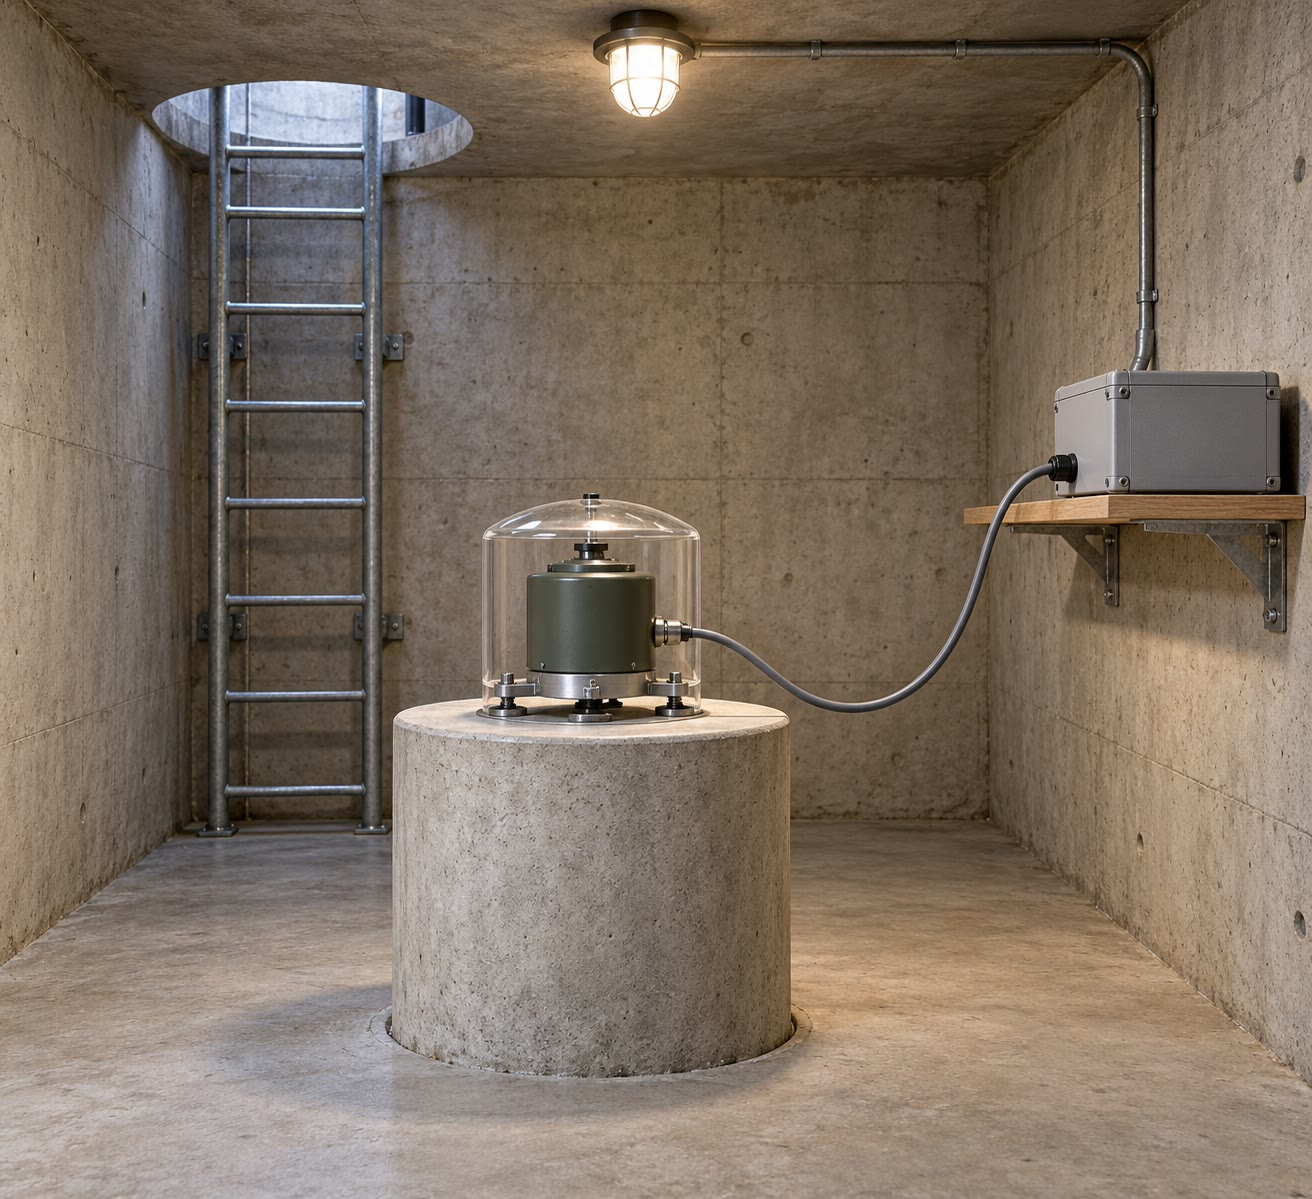
\includegraphics[width=\linewidth]{images/book3/ai/b1-seismometer-vault.jpg}

{\scriptsize مقياس زلازل عريض النطاق على رصيفه في حجرة تحت الأرض، ومسجّل البيانات على الجدار (رسم توضيحي مُولَّد بالذكاء الاصطناعي).}
\end{minipage}
\end{inthefield}

\section{التمارين}

\begin{exercise}[$\star$]\label{exo:b1:layered-earth:1}
بالنصفين القطريين ل PREM، $R = \qty{6371}{km}$، و$r_{\text{ل–و}} = \qty{3480}{km}$ و$r_{\text{ل–د}} = \qty{1221.5}{km}$، احسب كسري حجم الأرض اللذين يشغلهما اللب \omterm{def:b1:layered-earth:layers}{واللب الداخلي}.
% ledger: prem:cmb, prem:icb
\end{exercise}

\begin{exercise}[$\star$]\label{exo:b1:layered-earth:2}
مباشرةً فوق \omterm{def:b1:layered-earth:discontinuity}{حدّ اللب–الوشاح} تعطي PREM $v_P = \qty{13.7166}{km.s^{-1}}$، و$v_S = \qty{7.26466}{km.s^{-1}}$، و$\rho = \qty{5.56645}{g.cm^{-3}}$؛ ومباشرةً تحته، $v_P = \qty{8.06482}{km.s^{-1}}$، و$v_S = 0$، و$\rho = \qty{9.90349}{g.cm^{-3}}$. احسب \omterm{def:b1:layered-earth:seismic-parameter}{المعامل الزلزالي} ومعامل الحجم على كل جانب (بوحدة \unit{GPa}). ما الذي يتغيّر أكثر عبر الحدّ؟
% ledger: data:prem, prem:cmb
\end{exercise}

\begin{exercise}[$\star$]\label{exo:b1:layered-earth:3}
\omterm{def:b1:layered-earth:layers}{القشرة} سمكها \qty{30}{km}، بسرعة \qty{6.2}{km.s^{-1}}، تستند إلى \omterm{def:b1:layered-earth:layers}{الوشاح} بسرعة \qty{8.1}{km.s^{-1}}. احسب الزاوية الحرجة، والمسافة الحرجة، \omterm{def:b1:layered-earth:head-wave}{ومسافة التقاطع}.
\end{exercise}

\begin{exercise}[$\star$]\label{exo:b1:layered-earth:4}
كتلة اللب \qty{1.94e24}{kg} ونصف قطره \qty{3480}{km}. احسب الجاذبية عند \omterm{def:b1:layered-earth:discontinuity}{حدّ اللب–الوشاح} وقارنها بجاذبية السطح، \qty{9.82}{m.s^{-2}}. لماذا تكون أكبر؟
\end{exercise}

\begin{exercise}[$\star\star$]\label{exo:b1:layered-earth:5}
في مقطع انكسار تكون الوصلات الأولى عند \qty{10.0}{s} على \qty{60}{km}، وعند \qty{33.3}{s} على \qty{200}{km}، وعند \qty{45.8}{s} على \qty{300}{km}؛ والخط المار بالنقطة الأولى يمرّ بالأصل. اعثر على $v_1$ و$v_2$ وزمن القطع وعمق الحدّ، وتحقّق من النتيجة \omterm{def:b1:layered-earth:head-wave}{بمسافة التقاطع}.
\end{exercise}

\begin{exercise}[$\star\star$]\label{exo:b1:layered-earth:6}
بيّن أن الكرة المنتظمة لها $I = 0.4\,MR^2$. ثم احسب الكتلة ومعامل $I/MR^2$ لأرض من طبقتين: لبّ نصف قطره \qty{3480}{km} وكثافته \qty{11.0}{g.cm^{-3}} في \omterm{def:b1:layered-earth:layers}{وشاح} كثافته \qty{4.45}{g.cm^{-3}}، مع $R = \qty{6371}{km}$. قارن ب\num{5.972e24} kg وب$0.3308$.
\end{exercise}

\begin{exercise}[$\star\star$]\label{exo:b1:layered-earth:7}
على عمق \qty{1471}{km} تعطي PREM $v_P = \qty{12.16}{km.s^{-1}}$، و$v_S = \qty{6.673}{km.s^{-1}}$، و$\rho = \qty{4.86}{g.cm^{-3}}$، والجاذبية \qty{9.9}{m.s^{-2}}. احسب تدرّج الكثافة الذي تعطيه معادلة آدامز–ويليامسون، بوحدة \unit{g.cm^{-3}} لكل \qty{1000}{km}، وقارنه بكثافتي PREM، \num{4.844} عند \qty{1471}{km} و\num{5.357} عند \qty{2471}{km}.
% ledger: data:prem
\end{exercise}

\begin{exercise}[$\star\star$]\label{exo:b1:layered-earth:8}
قدّر الضغط عند عمق \qty{670}{km} من كثافة متوسطة قدرها \qty{3.57}{g.cm^{-3}} وجاذبية \qty{9.9}{m.s^{-2}}. ما تغيّر \omterm{def:b1:rock-forming-minerals:mineral}{المعدن} المتوقع هناك؟
% ledger: frost:mantle-transitions
\end{exercise}

\begin{exercise}[$\star\star$]\label{exo:b1:layered-earth:9}
الكثافة المتوسطة \omterm{def:b1:layered-earth:layers}{للب الخارجي} في PREM هي \qty{10.90}{g.cm^{-3}}؛ وعند \omterm{def:b1:layered-earth:discontinuity}{حدّ اللب الداخلي} تبلغ كثافته \qty{12.166}{g.cm^{-3}} فوقه و\qty{12.764}{g.cm^{-3}} تحته. (أ)~إذا كان الحديد عند الظروف نفسها أكثف من \omterm{def:b1:layered-earth:layers}{اللب الخارجي} بنسبة \qtyrange{5}{10}{\percent}، فأي مدى من الكثافات يعطي ذلك للحديد السائل هناك؟ (ب)~احسب قفزة الكثافة عند \omterm{def:b1:layered-earth:discontinuity}{حدّ اللب الداخلي} بالنسبة المئوية، وقارنها ب\qty{4.5}{\percent} من الدراسات الحديثة. (ج)~ماذا تعطي قفزة أكبر من التجمّد وحده عن العناصر الخفيفة؟
% ledger: badro:core, prem:icb
\end{exercise}

\begin{exercise}[$\star\star\star$]\label{exo:b1:layered-earth:10}
بيّن أن زمن الموجة المنعكسة $t_r(x) = \sqrt{x^2 + 4h^2}/v_1$ وزمن \omterm{def:b1:layered-earth:head-wave}{موجة الرأس} في \cref{thm:b1:layered-earth:two-layer} متساويان، ولهما الميل نفسه، عند $x = 2h\tan i_c$، وأن $t_r > t_{\text{الرأس}}$ بعدها. فسّر ذلك.
\end{exercise}

\begin{exercise}[$\star\star\star$]\label{exo:b1:layered-earth:11}
لأرض ذات كثافة منتظمة $\rho$، بيّن أن $g(r) = \tfrac43\pi G\rho r$ و$P(r) = \tfrac23\pi G\rho^2(R^2 - r^2)$. احسب الضغط المركزي ب$\rho = \qty{5513}{kg.m^{-3}}$ و$R = \qty{6371}{km}$، وقارنه ب\qty{363.85}{GPa} من PREM.
% ledger: earth:density, prem:centre
\end{exercise}

\begin{exercise}[$\star\star\star$]\label{exo:b1:layered-earth:12}
بيّن أنه إذا كان $g/\Phi$ ثابتًا عبر طبقة، فإن معادلة آدامز–ويليامسون تعطي $\rho = \rho_0\exp\bigl(g(z - z_0)/\Phi\bigr)$ مع العمق $z$. طبّقها على \omterm{def:b1:layered-earth:layers}{اللب الخارجي}، من \qty{2891}{km} ($\rho_0 =
\qty{9.90}{g.cm^{-3}}$) إلى \qty{5149.5}{km}، بالقيم المتوسطة $g = \qty{7.9}{m.s^{-2}}$ و$\Phi = \qty{87}{km^2.s^{-2}}$؛ وقارن بكثافة PREM، \qty{12.17}{g.cm^{-3}}، عند \omterm{def:b1:layered-earth:discontinuity}{حدّ اللب الداخلي}.
% ledger: prem:icb
\end{exercise}

\section{مسألة: وزن قشور الأرض}

\begin{problem}[{مسألة نهاية الأسبوع --- الحجوم والكتل وعزم القصور الذاتي لأرض من أربع قشور مبنية من PREM، مقارنةً بالكتلة وعزم القصور الذاتي المقيسين؛ الجاذبية والضغط في العمق}]
\label{pb:b1:layered-earth:1}
% values: calc/ch09.py; mean densities rounded from figdata prem_profiles (values part)
% ledger: data:prem, prem:constraints, prem:centre, prem:cmb, earth:mass, earth:MoI, const:G
قُطعت الأرض إلى أربع قشور عند أنصاف أقطار PREM، وأُعطيت كل \omterm{def:b1:layered-earth:layers}{قشرة} متوسط كثافتها في PREM، مقرّبًا:
\begin{center}
\small
\begin{tabular}{lccc}
\hline
\omterm{def:b1:layered-earth:layers}{القشرة} & من (km) & إلى (km) & متوسط الكثافة (\unit{g.cm^{-3}}) \\
\hline
\omterm{def:b1:layered-earth:layers}{القشرة} \omterm{def:b1:layered-earth:layers}{والوشاح} العلوي ومنطقة الانتقال & 5701 & 6371 & 3.57 \\
\omterm{def:b1:layered-earth:layers}{الوشاح} السفلي & 3480 & 5701 & 4.90 \\
\omterm{def:b1:layered-earth:layers}{اللب الخارجي} & 1221.5 & 3480 & 10.90 \\
\omterm{def:b1:layered-earth:layers}{اللب الداخلي} & 0 & 1221.5 & 12.89 \\
\hline
\end{tabular}
\end{center}
استعمل $G = \qty{6.674e-11}{m^3.kg^{-1}.s^{-2}}$. وكتلة الأرض المقيسة \qty{5.972e24}{kg}، ومعامل عزم القصور الذاتي $I/MR^2 = 0.3308$.

\medskip
\noindent\textbf{الجزء الأول --- الحجوم.}
\begin{enumerate}
  \item احسب حجم الأرض.
  \item احسب حجم كل \omterm{def:b1:layered-earth:layers}{قشرة}.
  \item ما كسر الحجم الذي تشغله كل \omterm{def:b1:layered-earth:layers}{قشرة}؟ أيّ القشور أكبرها؟
  \item ما كسر الحجم الذي يشغله اللب؟
\end{enumerate}

\noindent\textbf{الجزء الثاني --- الكتل.}
\begin{enumerate}[resume]
  \item احسب كتلة كل \omterm{def:b1:layered-earth:layers}{قشرة}.
  \item اجمعها، وقارن المجموع بالكتلة المقيسة.
  \item استنتج متوسط كثافة الأرض النموذجية.
  \item ما كسر الكتلة الموجود في \omterm{def:b1:layered-earth:layers}{اللب الداخلي}؟
  \item ما كسر الكتلة الموجود في \omterm{def:b1:layered-earth:layers}{الوشاح} \omterm{def:b1:layered-earth:layers}{والقشرة} معًا؟
  \item قارن حصة اللب من الحجم ومن الكتلة، واشرح.
\end{enumerate}

\noindent\textbf{الجزء الثالث --- عزم القصور الذاتي.}
\begin{enumerate}[resume]
  \item بيّن من \cref{prop:b1:layered-earth:integrals} أن \omterm{def:b1:layered-earth:layers}{قشرة} منتظمة بين $r_1$ و$r_2$ لها $I = \tfrac{8\pi}{15}\rho\,(r_2^5 - r_1^5)$.
  \item احسب عزم القصور الذاتي لكل \omterm{def:b1:layered-earth:layers}{قشرة}.
  \item أيّ القشور تسهم أكثر، ولماذا يسهم \omterm{def:b1:layered-earth:layers}{اللب الداخلي} بما يقارب الصفر؟
  \item اجمعها واحسب $I/MR^2$ للنموذج.
  \item قارن ب$0.3308$ وب$0.4$ للكرة المنتظمة.
  \item داخل كل \omterm{def:b1:layered-earth:layers}{قشرة} حقيقية تزداد الكثافة مع العمق. هل يفسّر ذلك لماذا يكون معامل النموذج مرتفعًا أكثر من اللازم؟ اشرح.
\end{enumerate}

\noindent\textbf{الجزء الرابع --- الجاذبية والضغط.}
\begin{enumerate}[resume]
  \item احسب الجاذبية عند سطح النموذج.
  \item احسب الجاذبية عند \omterm{def:b1:layered-earth:discontinuity}{حدّ اللب–الوشاح}.
  \item احسب متوسط كثافة \omterm{def:b1:layered-earth:layers}{الوشاح} \omterm{def:b1:layered-earth:layers}{والقشرة} معًا.
  \item الجاذبية في \omterm{def:b1:layered-earth:layers}{الوشاح} تبقى قرب \qty{10}{m.s^{-2}}. قدّر الضغط عند \omterm{def:b1:layered-earth:discontinuity}{حدّ اللب–الوشاح}، وقارنه ب\qty{135.75}{GPa} من PREM.
  \item احسب متوسط كثافة اللب، وزيادة الضغط من \omterm{def:b1:layered-earth:discontinuity}{حدّ اللب–الوشاح} حتى المركز في لب منتظم، $\tfrac23\pi G\rho_c^2 r_c^2$ (\cref{exo:b1:layered-earth:11} مطبّقًا على اللب وحده).
  \item اجمع الاثنين لتقدير الضغط المركزي، وقارنه ب\qty{363.85}{GPa} من PREM. لماذا يكون التقدير منخفضًا؟
  \item أيّ أرقام النموذج تُقارن بقياس، وأيّها يُقارَن بنموذج PREM نفسه وحده؟
  \item ما كسر كتلة الأرض الموجود في اللب؟
\end{enumerate}
\end{problem}
